\documentclass[10pt,a4paper]{article}
\usepackage[utf8]{inputenc}
\usepackage[english]{babel}
\usepackage{amsmath}
\usepackage{amsfonts}
\usepackage{amssymb}
\usepackage{graphicx}
\title{COS 301 Software Documentation}
\author{Dieter Doman 11002566 \\
		Melany Barnes 12030466 \\
		Rudiger Roach 11004322 \\
		Johan Esterhuyse 10043285}
\date{}
\begin{document}
  \begin{center}
  \advance\leftskip-5.0cm
	
\includegraphics{Pictures/TopBorder.png}
  \end{center}
\maketitle
\begin{center}
Version 1.0 \\
GitHub link: https://github.com/RudigerRoach/301\textunderscore main\textunderscore emma.git \\
\vspace*{5\baselineskip}
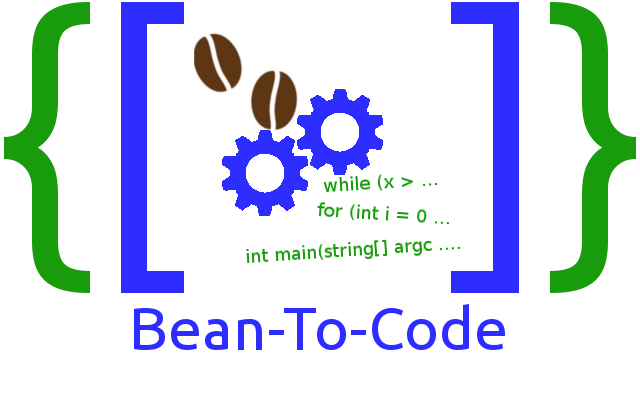
\includegraphics[scale=0.5]{Pictures/Logo.png}
\end{center}
  \begin{center}
  \advance\leftskip-5.0cm
	
\includegraphics{Pictures/BottomBorder.png}
  \end{center}
\pagebreak
\tableofcontents
\pagebreak
\section{Overview, Vision and Scope}
\section{Architecture requirements}
\section{Functional requirements and application design}
\subsection{Introduction}
\subsection{Required Functionality}
\subsubsection{Functional requirements for registration and login}
A first time user will be required to register by filling in his/her email address and password, as well as confirm password.
To login for the first time a user will have to enter his/her email address and password. The credentials provided will be tested against the database to determine if it is valid.  If login fails the user will be directed to the register screen. If login is successful the device's unique identifier will be sent to the server to remember the device on the system. The user will then be able to use the rest of the system.

\subsection{Use case prioritization}
\subsection{Use case/Services contracts}
\subsection{Process specifications}
Activity sequence diagrams
\subsection{Domain objects}
\section{Glossary}
\end{document}